\documentclass[tikz,border=10pt]{standalone}
\usepackage{tikz}

\begin{document}

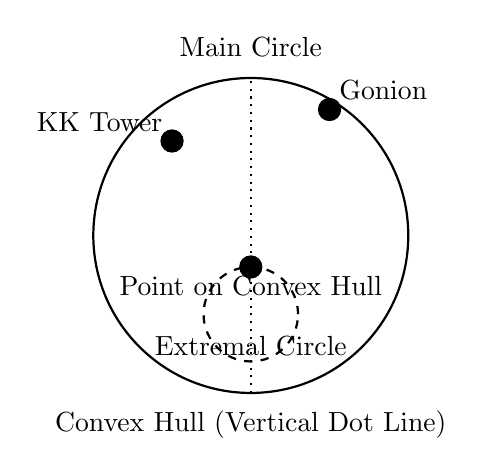
\begin{tikzpicture}[scale=2]
    % Draw the main circle
    \draw[thick] (0,0) circle (1);
    
    % Draw the vertical dot line (convex hull)
    \draw[dotted, thick] (0,-1) -- (0,1);
    
    % Draw the extremal circle
    \draw[dashed, thick] (0,-0.5) circle (0.3);
    
    % Add labels
    \node at (0,1.2) {Main Circle};
    \node at (0,-1.2) {Convex Hull (Vertical Dot Line)};
    \node at (0,-0.7) {Extremal Circle};
    
    % Add points for clarity
    \filldraw (0.5,0.8) circle (2pt) node[above right] {Gonion};
    \filldraw (-0.5,0.6) circle (2pt) node[above left] {KK Tower};
    \filldraw (0,-0.2) circle (2pt) node[below] {Point on Convex Hull};
\end{tikzpicture}

\end{document}